\section{Implementacja w języku C++}
\subsection{Proces projektowania}
Cechy środowiska Matlab ułatwiają przeprowadzenie procesu prototypowania i wstępnego testowania aplikacji, co jednak nie jest równoznaczne aspektom koniecznym do zaprojektowania możliwie najwydajniejszej i stabilnej aplikacji klasyfikującej sygnał $EKG$. Z tego względu, po zakończeniu procesu prototypowania zaprojektowano program w języku C++, wykorzystujący badane algorytmy. W trakcie pracy wykorzystano bibliotekę $Eigen$, oferującą wydajną implementację operacji arytmetycznych na macierzach. Użyto również biblioteki $IGL$ \cite{libigl-www}, oferującej szereg funkcji dostępnych w środowisku Matlab oraz interfejsu $OpenMP$ \cite{openmp-www}, umożliwiającego tworzenie programów wykorzystujących zalety systemów wieloprocesorowych.

Zaprojektowany program był w pełni kompatybilny z przygotowanymi prototypami algorytmów, wyniki klasyfikacji oraz cechy nie odbiegały od danych uzyskanych w środowisku Matlab. Dzięki zrównolegleniu sekcji odpowiedzialnych za klasyfikację wektorów testowych osiągnięto kilkukrotnie większą wydajność względem prototypu. Wyniki zebrano w tabeli \ref{matlab-vs-cpp-time}.

\begin{table}[H]
	\centering
	\begin{tabular}{|c|r|r|r|r|}
		\hline
		Plik & KNN Matlab & KNN C++ & ENN Matlab & ENN C++  \\ 
\hline
$100$ & 0.0530 & 0.0203 & 0.1356 & 0.0329 \\
\hline
$101$ & 0.0175 & 0.0109 & 0.0572 & 0.0141 \\
\hline
$102$ & 0.0164 & 0.0109 & 0.0489 & 0.0095 \\
\hline
$103$ & 0.0161 & 0.0084 & 0.0617 & 0.0097 \\
\hline
$104$ & 0.0072 & 0.0035 & 0.0265 & 0.0043 \\
\hline
$105$ & 0.0837 & 0.0227 & 0.2662 & 0.0557 \\
\hline
$106$ & 0.0385 & 0.0119 & 0.1135 & 0.0218 \\
\hline
$108$ & 0.0015 & 0.0013 & 0.0072 & 0.0015 \\
\hline
$109$ & 0.0123 & 0.0059 & 0.0351 & 0.0087 \\
\hline
$111$ & 0.0064 & 0.0039 & 0.0148 & 0.0051 \\
\hline
$112$ & 0.0906 & 0.0298 & 0.2721 & 0.0691 \\
\hline
$113$ & 0.0213 & 0.0083 & 0.0616 & 0.0134 \\
\hline
$118$ & 0.0015 & 0.0019 & 0.0041 & 0.0014 \\
\hline
$119$ & 0.0265 & 0.0090 & 0.0771 & 0.0148 \\
\hline
$121$ & 0.0163 & 0.0067 & 0.0413 & 0.0099 \\
\hline
$122$ & 0.0631 & 0.0169 & 0.1756 & 0.0380 \\
\hline
$124$ & 0.0225 & 0.0075 & 0.0656 & 0.0119 \\
\hline
$200$ & 0.0049 & 0.0028 & 0.0107 & 0.0032 \\
\hline
$201$ & 0.0021 & 0.0012 & 0.0041 & 0.0013 \\
\hline
$202$ & 0.0127 & 0.0056 & 0.0332 & 0.0078 \\
\hline
$203$ & 0.0434 & 0.0137 & 0.1157 & 0.0243 \\
\hline
$205$ & 0.0577 & 0.0180 & 0.1771 & 0.0394 \\
\hline
$208$ & 0.0272 & 0.0100 & 0.0850 & 0.0264 \\
\hline
$209$ & 0.0073 & 0.0043 & 0.0173 & 0.0055 \\
\hline
$210$ & 0.0941 & 0.0274 & 0.3368 & 0.0713 \\
\hline
$212$ & 0.0159 & 0.0068 & 0.0433 & 0.0101 \\
\hline
$213$ & 0.1775 & 0.0439 & 0.5610 & 0.1048 \\
\hline
$214$ & 0.0064 & 0.0042 & 0.0166 & 0.0051 \\
\hline
$215$ & 0.0137 & 0.0064 & 0.0366 & 0.0097 \\
\hline
$217$ & 0.0033 & 0.0026 & 0.0082 & 0.0030 \\
\hline
$219$ & 0.0548 & 0.0210 & 0.1791 & 0.0352 \\
\hline
$221$ & 0.0084 & 0.0046 & 0.0234 & 0.0062 \\
\hline
$222$ & 0.0602 & 0.0174 & 0.1918 & 0.0350 \\
\hline
$223$ & 0.0015 & 0.0014 & 0.0050 & 0.0015 \\
\hline
$228$ & 0.0359 & 0.0117 & 0.1099 & 0.0230 \\
\hline
$231$ & 0.0522 & 0.0157 & 0.1629 & 0.0304 \\
\hline
$233$ & 0.0490 & 0.0159 & 0.1503 & 0.0332 \\
\hline
$234$ & 0.1096 & 0.0310 & 0.3523 & 0.0702 \\
\hline	
	\end{tabular}
	\caption{Porównanie czasu działania w sekundach dla algorytmów zaprojektowanych w Matlabie i C++.}
	\label{tab:matlab-vs-cpp-time}	
\end{table}
Algorytm $KNN$ zaprojektowany w języku C++ wykonywał się średnio $2.45$ razy szybciej od prototypu w Matlabie, natomiast algorytm $ENN$ - średnio $4.38$ razy szybciej. $ENN$ wymaga ponadto średnio o $76\%$ więcej czasu od $KNN$ na przeprowadzenie obliczeń dla tego samego zbioru danych.

\subsection{Wpływ rozmiaru badanych zbiorów na wydajność aplikacji}
Algorytm $KNN$ wymaga analizy pełnego zbioru uczącego dla każdego badanego wektora. Czas wykonania aplikacji zależy więc w sposób liniowy zarówno od rozmiaru obu zbiorów. W przypadku analizy danych poprzez podział zbioru na zbiór uczący i testowy ze stałym współczynnikiem, czas potrzebny na przeprowadzenie obliczeń zależy kwadratowo od wielkości zbioru wejściowego.

Proces uczenia w przypadku algorytmu $ENN$ wymaga przeprowadzenia obliczeń zależnych liniowo od wielkości zbioru uczącego oraz liczby unikalnych klas. Czas wymagany do przeprowadzenia klasyfikacji zależy liniowo od liczności zbioru testowego oraz liczby wektorów uczących.

Złożoność obliczeniowa obu algorytmów zdominowana jest przez wielkość zbiorów uczącego i testowego. Na etapie testowania aplikacji założono, że relacja pomiędzy wielkością zbiorów jest stała. Czasowa złożoność obliczeniowa w takim przypadku opisana być może pewną funkcją kwadratową, której argumentem jest wielkość zbioru na wejściu aplikacji.
Na rysunkach \ref{fig:knn_compexity} i \ref{fig:enn_complexity} przedstawiono dane eksperymentalne z działania algorytmów na zbiorach różnych rozmiarów.

\begin{figure}[H]
	\centering
	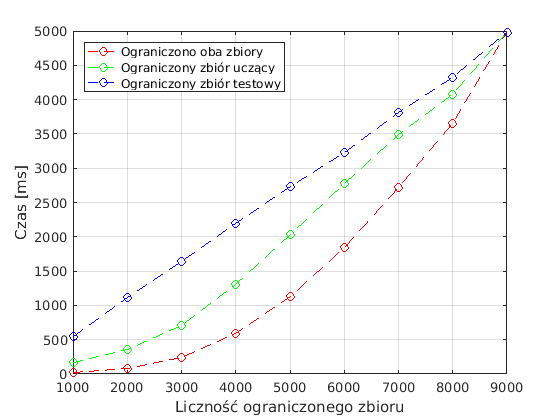
\includegraphics[width=14cm]{img/knn_compexity}
	\caption{Czasowa złożoność obliczeniowa algorytmu $KNN$.}
	\label{fig:knn_compexity}
\end{figure}
\begin{figure}[H]
	\centering
	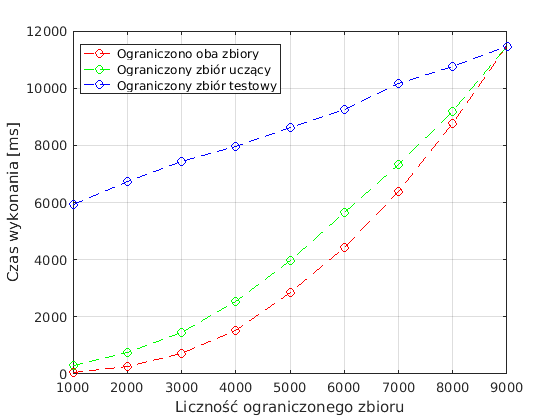
\includegraphics[width=14cm]{img/enn_complexity}
	\caption{Czasowa złożoność obliczeniowa algorytmu $KNN$.}
	\label{fig:enn_complexity}
\end{figure}

W trakcie eksperymentu manipulowano licznością zbioru testowego oraz uczącego. Badano działanie aplikacji dla zmiennej wielkości jednego zbioru przy stałym rozmiarze drugiego równym $9000$ oraz dla zbiorów o takiej samej wielkości w zakresie od $1000$ do $9000$ wektorów. W przypadku obu algorytmów zaobserwować można liniowy wzrost czasu wykonania przy manipulacji rozmiarem jednego zbioru oraz kwadratowy wzrost w przypadku zmiany wielkości obu zbiorów jednocześnie.

Badano możliwość redukcji zbioru uczącego w taki sposób, aby zawierał on taką samą liczbę wektorów dla każdej klasy. Proponowane rozwiązanie pozwala na ograniczenie czasu potrzebnego na przeprowadzenie procesu klasyfikacji, wymaga jednak przygotowania reprezentatywnego zbioru uczącego. Badano możliwość generowania zredukowanego zbioru uczącego przy starcie aplikacji lecz zaobserwowano znaczny spadek skuteczności algorytmów klasyfikacji. 

Zbadano również wpływ wielkości zbioru uczącego na podstawie analizy danych zawierających 32812 wektorów testowych. Wyniki zebrano w tabeli \ref{tab:rozmiar-zbioru-uczacego}.

\begin{table}[H]
	\centering
	\begin{tabular}{|r|r|r|r|r|}
		\hline
		Wielkość zbioru uczącego & Sk. KNN [\%] & Czas KNN [s] & Sk. ENN [\%] & Czas ENN [s]  \\ 
		\hline
		0.1 & 72.82 & 3.066 & 75.93 & 3.950\\
		\hline
		0.2 & 73.18 & 11.754 & 67.52 & 14.505 \\
		\hline
		0.3 & 76.94 & 17.055 & 70.69 & 25.430 \\
		\hline
		0.4 & 80.10 & 19.466 & 74.14 & 34.135 \\
		\hline
		0.5 & 82.24 & 20.552 & 75.75 &  44.992\\
		\hline
		0.6 & 88.80 & 21.104 & 85.01 & 56.602 \\
		\hline
		0.7 & 96.18 & 17.040 & 93.68 & 63.049 \\
		\hline
		0.8 & 95.61 & 14.335 & 92.62 & 78.166 \\
		\hline
		0.9 & 96.34 & 8.333 & 94.14 & 86.396 \\
		\hline
	\end{tabular}
	\caption{Porównanie skuteczności i czasu działania aplikacji dla zbiorów uczących i testowych różnych wielkości.}
	\label{tab:rozmiar-zbioru-uczacego}	
\end{table}
W kolejnych krokach badano działanie obu metod przy użyciu zbioru uczącego zwierającego zdefiniowaną w pierwszej kolumnie tabeli część wszystkich danych. Pozostałe wektory trafiały do zbioru testowego. Zaobserwowano wzrost skuteczności obu algorytmów wraz ze wzrostem wielkości zbioru uczącego do wartości $0.7$. W obu przypadkach nie zauważono znaczących zmian skuteczności dla wartości z zakresu $0.7-0.9$. Na podstawie omawianych danych można stwierdzić, że czas wykonania algorytmu $ENN$ zależy w większym stopniu od rozmiaru zbioru uczącego niż testowego. Wynika to z nietrywialnego procesu uczenia klasyfikatora. W przypadku algorytmu $KNN$ zaobserwowano mniejsze wartości czasu wykonania w końcowej fazie eksperymentu.
\subsection{Wskaźniki jakości klasyfikatora}

Dla uzyskanych wyników klasyfikacji zostały wyznaczone wskaźniki jakości takie jak czułość i swoistość. Czułość określa w tym przypadku zdolność algorytmu do wykrycia choroby, czyli dla czułości równej 1, algorytm potrafi w każdym przypadku poprawnie wykryć chorobę. Swoistość określa zdolność algorytmu do poprawnej klasyfikacji osób zdrowych. Wskaźniki opisują jedynie zdolność klasyfikacji zdrowy/chory, nie bada jednak klasyfikacji pomiędzy poszczególne choroby. 
\newline
Wskaźniki obliczane są według następujących wzorów:

\begin{equation}
czulosc = \frac{Tp}{Tp+Fn}
\end{equation}

\begin{equation}
swoistosc = \frac{Tn}{Tn+Fp}
\end{equation}
\newline
TP – True Positive – liczba obserwacji poprawnie zaklasyfikowanych do klasy pozytywnej
\newline
TN – True Negative – liczba obserwacji poprawnie zaklasyfikowanych do klasy negatywnej
\newline
FP – False Positive – liczba obserwacji zaklasyfikowanych do klasy pozytywnej podczas, gdy w rzeczywistości pochodzą z klasy negatywnej
\newline
FN – False Negative – liczba obserwacji zaklasyfikowanych do klasy negatywnej podczas, gdy w rzeczywistości pochodzą z klasy pozytywnej


Dla niektórych plików obliczenie wskaźników nie było możliwe, ze względu na zerową wartość sumy znajdującej się w mianowniku. Jest to spowodowane m.in występowaniem tylko jednej klasy w niektórych plikach. W takim przypadku wszystkie próbki klasyfikowane są jako występujaca klasa, a skuteczność działania wynosi 100\%.

\begin{table}[H]
	\centering
	\begin{tabular}{|c|r|r|r|r|}
		\hline
		& \multicolumn{2}{c|}{$kNN$} & \multicolumn{2}{c|}{$eNN$} \\
		\hline
		$Plik$ & Czułość & Swoistość & Czułość & Swoistość \\
		\hline
100 &1 &1 &0.85714 &1\\                  
\hline                                   
101 &--- &1 &--- &0.9951\\               
\hline                                   
102 &0.99451 &--- &1 &---\\              
\hline                                   
103 &--- &1 &--- &1\\                    
\hline                                   
104 &0.9625 &0.9375 &0.9625 &0.9375\\    
\hline                                   
105 &0.5 &1 &0.5 &0.99795\\              
\hline                                   
106 &0.96721 &1 &0.96721 &1\\            
\hline                                   
108 &0 &1 &0 &1\\                        
\hline                                   
109 &1 &--- &1 &---\\                    
\hline                                   
111 &1 &--- &1 &---\\                    
\hline                                   
112 &--- &1 &--- &1\\                    
\hline                                   
113 &0 &1 &1 &0.98684\\                  
\hline                                   
118 &1 &--- &1 &---\\                    
\hline                                   
119 &0.86667 &1 &0.86667 &1\\            
\hline                                   
121 &--- &1 &--- &1\\                    
\hline                                   
122 &--- &1 &--- &1\\                    
\hline                                   
124 &1 &--- &1 &---\\                    
\hline                                   
200 &0.5 &1 &1 &0.97059\\                
\hline                                   
201 &0 &1 &0.071429 &1\\                 
\hline                                   
202 &--- &0.99371 &--- &0.93082\\        
\hline                                   
203 &--- &1 &--- &1\\                    
\hline                                   
205 &0 &1 &0 &1\\                        
\hline                                   
208 &0.85 &0.97166 &0.85 &0.92713\\      
\hline                                   
209 &0.44444 &0.98165 &0.88889 &0.9633\\ 
\hline                                   
210 &0 &1 &0 &0.99819\\                  
\hline                                   
212 &1 &1 &1 &1\\                        
\hline                                   
213 &0.77419 &0.98085 &0.80645 &0.94256\\
\hline                                   
214 &1 &--- &1 &---\\                    
\hline                                   
215 &1 &1 &1 &1\\                        
\hline                                   
217 &0.80952 &1 &0.80952 &1\\            
\hline                                   
219 &0 &1 &0 &0.978\\                    
\hline                                   
221 &1 &0.99187 &1 &0.99187\\            
\hline                                   
222 &0.7 &0.90598 &0.86667 &0.81766\\    
\hline                                   
223 &0.90625 &--- &0.90625 &---\\        
\hline                                   
228 &0.95 &1 &0.95 &0.9924\\             
\hline                                   
231 &0.99698 &0.98 &0.99698 &1\\         
\hline                                   
233 &0.85714 &1 &0.85714 &0.99467\\      
\hline                                   
234 &--- &1 &--- &1\\                    
\hline                                   
	\end{tabular}
	\caption{Czułość i swoistość algorytmu kNN i eNN.}
	\label{tab:matlab-wskazniki}
\end{table}
\subsection{Omówienie możliwości wykorzystania zrównoważonego zbioru uczącego?}

\subsection{Rozkład danych w zbiorze uczącym i testowym.}
W rozdziale \ref{chap:prototype} została przedstawiona skuteczność działania algorytmu dla różnych plików. W tym rozdziale zostaną omówione rozkłady klas w niektórych plikach, oraz ich wpływ na działanie algorytmu.


W tabeli \ref{tab:matlab-plik100} został przedstawiony rozkład klas w pliku 100. W pliku występują dwie klasy 1 i 3. Pomimo bardzo dużej różnicy pomiędzy licznością obu klas podczas klasyfikacji za pomocą metody eNN tylko jedna próbka została źle sklasyfikowana, natomiast algorytm kNN był bezbłędny. W tym przypadku 10 próbek z klasy 3 wystarcza do przeprowadzenia poprawnego procesu uczenia algorytmów.

\begin{table}[H]
	\centering
	\begin{tabular}{|c|r|r|r|r|}
		\hline
		
		Klasa & Zbiór uczący & Zbiór testowy & Klasyfikacja kNN & Klasyfikacja eNN \\
		\hline
		1 & 737 & 314 & 314 & 315 \\
		\hline 
		3 & 10 & 7 & 7 & 6 \\
		\hline
                          
	\end{tabular}
	\caption{Szczegółowy rozkład klas dla pliku 100}
	\label{tab:matlab-plik100}
\end{table}

W przypadku pliku 204 algorytm eNN zaklasyfikował 6 próbek do klasy 3 pomimo iż takie w zbiorze testowym nie występowały. W przypadku algorytmu eNN wystąpienie stosunkowo dużej ilości klasyfikacji typu \textit{false positive} może zachodzić dla klas o małej liczebności w zbiorze uczącym co nastąpiło w tym przypadku.

\begin{table}[H]
	\centering
	\begin{tabular}{|c|r|r|r|r|}
		\hline
		
		Klasa & Zbiór uczący & Zbiór testowy & Klasyfikacja kNN & Klasyfikacja eNN \\
		\hline
		1 & 61 & 16 & 18 & 18 \\
		\hline 
		3 & 3 & 0 & 0 & 6 \\
		\hline
		4 & 159 & 80 & 78 & 72 \\
		\hline
		
	\end{tabular}
	\caption{Szczegółowy rozkład klas dla pliku 104}
	\label{tab:matlab-plik104}
\end{table}


W tabeli \ref{tab:matlab-skutecznosc} opisującej skuteczność działania algorytmów zdecydowanie wyróżniają się wyniki uzyskane dla pliku 201. W tabeli \ref{tab:matlab-plik201} został przedstawiony rozkład klas w tym pliku. Niska skuteczność działania algorytmu wynika ze źle przygotowanego zbioru uczącego, w którym nie znalazły się próbki z klas 3 i 7 co uniemożliwiło ich poprawną klasyfikację. Dodatkową przeszkodą była niska liczebność zbioru co wiąże się z małą ilością próbek poszczególnych klas.

\begin{table}[H]
	\centering
	\begin{tabular}{|c|r|r|r|r|}
		\hline
		
		Klasa & Zbiór uczący & Zbiór testowy & Klasyfikacja kNN & Klasyfikacja eNN \\
		\hline
		1 & 66 & 15 & 29 & 28 \\
		\hline 
		3 & 0 & 8 & 0 & 0 \\
		\hline
		4 & 1 & 0 & 0 & 1 \\
		\hline
		7 & 0 & 6 & 0 & 0 \\
		\hline
		
	\end{tabular}
	\caption{Szczegółowy rozkład klas dla pliku 201}
	\label{tab:matlab-plik201}
\end{table}




